% \documentclass{beamer}

% \usepackage{graphicx}
% \usepackage{wrapfig}

% \title{Chapter 1 Storyboard: Climate Variability and Network Resilience}
% \author{}
% \date{}

% \begin{document}

% \frame{\titlepage}

% % ------------------------------------------------
% \begin{frame}{Main Questions}
% \begin{itemize}
%     \item How does climate variability (precipitation, temperature) shape plant–pollinator network structure?
%     \item Do climate-driven structural changes alter network robustness and community resistance?
%     \item Does the mechanism of species loss (extinction scenario) mediate climate effects on robustness?
% \end{itemize}
% \end{frame}

% % ------------------------------------------------
% \begin{frame}{Study Motivation}
% \begin{itemize}
%     \item Climate variability is a key driver of instability.
%     \item Plant-pollinator networks are sensitive because interactions depend on species and phenology.
%     \item Network structure (complementarity, redundancy, specialization, richness) mediates resilience.
%     \item Loss of interactions triggers cascading extinctions.
%     \item Robustness is the key metric linking structure and species loss to resilience.
%     \item Sky Island mountain meadows are biodiversity hotspots that provide a natural climate gradient.
%     \item Climate variability reshapes networks via species turnover, interaction frequency, and phenological shifts.
% \end{itemize}
% \end{frame}

% % ------------------------------------------------
% \begin{frame}{Network Concepts: Resistance, Robustness, Resilience}
% \begin{itemize}
%     \item \textbf{Resistance:} 
%     Immediate structural response to environmental change  
%     \begin{itemize}
%         \item Measured as deviation from baseline network structure
%         \item Captures sensitivity to climate variability
%     \end{itemize}

%     \item \textbf{Robustness:} 
%     Persistence of the network under sequential species loss  
%     \begin{itemize}
%         \item Measured using coextinction simulations
%         \item Captures tolerance to disturbance
%     \end{itemize}

%     \item \textbf{Resilience:} 
%     Ability to recover after disturbance  
%     \begin{itemize}
%         \item Not directly measured here
%         \item Inferred conceptually from resistance + robustness
%     \end{itemize}

%     \item \textbf{Key distinction:}
%     Resistance reflects \emph{short-term change}, while robustness reflects \emph{persistence under species loss}.
% \end{itemize}
% \end{frame}

% % ------------------------------------------------
% \begin{frame}{Conceptual Framework}
% \begin{figure}
%         \centering
%         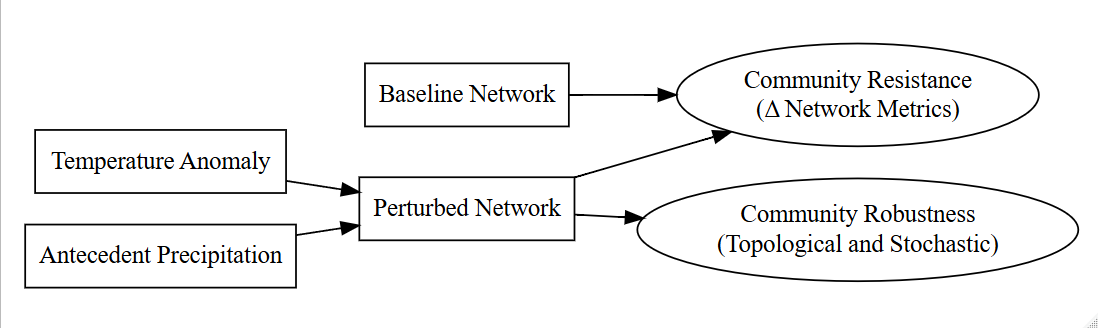
\includegraphics[width=1\linewidth]{SEM_diagram.png}
%     \end{figure}
% \begin{itemize}
%     \item Climate variability (temperature + precipitation) acts as environmental forcing.
%     \item Forcing is expected to alter interaction structure.
%     \item Structural changes influence ecological resilience.
%     \item Resistance = immediate structural response to climate.
%     \item Robustness = persistence under sequential species loss.
%     \item Overall pathway: climate $\rightarrow$ structure $\rightarrow$ resilience.
% \end{itemize}
% \end{frame}

% % ------------------------------------------------
% \begin{frame}{Methods}
% \begin{itemize}
%     \item 5 years of plant--pollinator networks across 11 Sky Island sites.
%     \item Climate predictors derived from daily PRISM data.
%     \item \textbf{Antecedent precipitation (APi)}: exponentially weighted cumulative rainfall prior to sampling; proxy for soil moisture and floral resource availability.
%     \item \textbf{Seasonal temperature anomaly:} cumulative deviation from long-term monthly normals from May 1 to each sample round; captures relative warmth or coolness of the season. 
%     \item \textbf{Community resistance: }proportional change in network metrics (complementarity, redundancy, specialization, richness) between baseline and perturbed conditions. 
%     \item \textbf{Network robustness:} coextinction simulations (TCM and SCM).
%     \item Mixed models include site and year as random effects.
% \end{itemize}
% \end{frame}

% % ------------------------------------------------
% \begin{frame}{Community Resistance \& Precipitation (Figure 3)}
% \begin{itemize}
%     \begin{figure}
%         \centering
%         \includegraphics[width=0.9\linewidth]{CommunityResistance_APi.pdf}
%     \end{figure}
%     \item Pollinator redundancy and plant generalization decrease under wetter conditions, others show no relationship.
%     \item Patterns suggest shifts toward more specialized interaction structure, though effects are modest.
% \end{itemize}
% \vspace{0.5cm}
% \end{frame}

% % ------------------------------------------------
% \begin{frame}{Community Resistance \& Temperature (Figure 4)}
% \begin{itemize}
%     \begin{figure}
%     \centering
%     \includegraphics[width=0.9\linewidth]{CommunityResistance_WindowTmeanAnom.pdf}
%     \end{figure}
%     \item Effects are generally weak and inconsistent; associations are mainly positive; temperature alone is a poor predictor of resistance, with site- and year-level variation dominating.
% \end{itemize}
% \end{frame}

% % =================================================
% \begin{frame}{Coextinction Models: Measuring Robustness}
% \begin{itemize}
%     \item \textbf{Topological Coextinction Model (TCM):}
%     \begin{itemize}
%         \item Species go extinct when all interaction partners are lost
%         \item Deterministic: extinction based on network structure alone
%         \item Emphasizes structural vulnerability
%     \end{itemize}

%     \item \textbf{Stochastic Coextinction Model (SCM):}
%     \begin{itemize}
%         \item Extinction occurs probabilistically based on interaction loss
%         \item Allows partial dependence on partners
%         \item Incorporates ecological uncertainty and variability
%     \end{itemize}

%     \item \textbf{Key difference:}
%     \begin{itemize}
%         \item TCM = strict structural collapse
%         \item SCM = probabilistic, more ecologically realistic responses
%     \end{itemize}

%     \item \textbf{Why both?}
%     \begin{itemize}
%         \item Compare how extinction assumptions influence robustness estimates
%         \item Test whether climate effects depend on disturbance dynamics
%     \end{itemize}
% \end{itemize}
% \end{frame}

% % =================================================
% \begin{frame}{TCM Robustness (Figure 1)}
% \begin{itemize}
%     \begin{figure}
%         \centering
%         \includegraphics[width=1\linewidth]{TCM_Robustness_by_climate.pdf}
%     \end{figure}
%     \[ \text{Robustness} \sim \text{APi} + \text{TmeanAnom} + (1 \mid \text{Site}) \]
%     \item Removed Year effect (no detectable temporal variance in some scenarios)
%     \item Climate effects are weak overall (marginal $R^2 \approx 0.02$–$0.19$)
%     \item \textbf{Take-home:} Climate sensitivity depends on extinction structure—strongest when highly connected or abundant species are removed first.
% \end{itemize}
% \end{frame}

% % ------------------------------------------------
% \begin{frame}{SCM Robustness (Figure 2)}
% \begin{itemize}
%     \begin{figure}
%         \centering
%         \includegraphics[width=1\linewidth]{SCM_Robustness_by_climate.pdf}
%     \end{figure}
%     \[ \text{Robustness} \sim \text{APi} + \text{TmeanAnom} + (1 \mid \text{Site}) + (1 \mid \text{Year}) \]
%     \item Both Site and Year effects retained (small but non-zero temporal variance)
%     \item Climate effects are weak (marginal $R^2 \approx 0.06$–$0.13$)
%     \item \textbf{Take-home:} SCM shows similar but slightly stronger climate effects, indicating results are robust to assumptions about extinction dynamics.
% \end{itemize}
% \end{frame}

% % =================================================
% \begin{frame}{Results Summary}
% \begin{itemize}
%     \item Higher antecedent precipitation was associated with slightly lower pollinator redundancy and plant generalization, suggesting that wetter conditions may promote more specialized interaction structures.
%     \item Climate variables explain a modest proportion of variation in robustness, with effects varying across extinction scenarios.
%     \item Precipitation shows consistent positive effects, but climate sensitivity is strongest when key species (high abundance or degree) are removed.
%     \item Temperature effects are generally weak.
%     \item Site- and year-level random effects explain substantial variance (microclimate, phenology, community composition) as important modulators of climate–network relationships.
% \end{itemize}
% \end{frame}

% % ------------------------------------------------
% \begin{frame}{Discussion: Biological Interpretation \& Implications}
% \begin{itemize}
%     \item Climate effects are real but context-dependent. 

%     \item Water availability likely operates through resource dynamics, increasing floral resources and potentially increasing interaction strength, temporal overlap, specialized interactions

%     \item Robustness is most climate-sensitive when highly connected or dominant species are removed.

%     \item Site-level differences (e.g., microclimate, community composition) explain more variation than year-to-year climate fluctuations.

%     \item Weak and inconsistent resistance responses suggest that immediate structural change and long-term robustness capture different dimensions of resilience.

%     \item \textbf{Implication:}
%     Predicting ecological responses to climate change requires accounting for both interaction structure and disturbance pathways, not just species richness or climate alone.
% \end{itemize}
% \end{frame}

% % % ------------------------------------------------
% % \begin{frame}{Revisiting the Conceptual Model}

% % \begin{figure}
% % \centering
% % 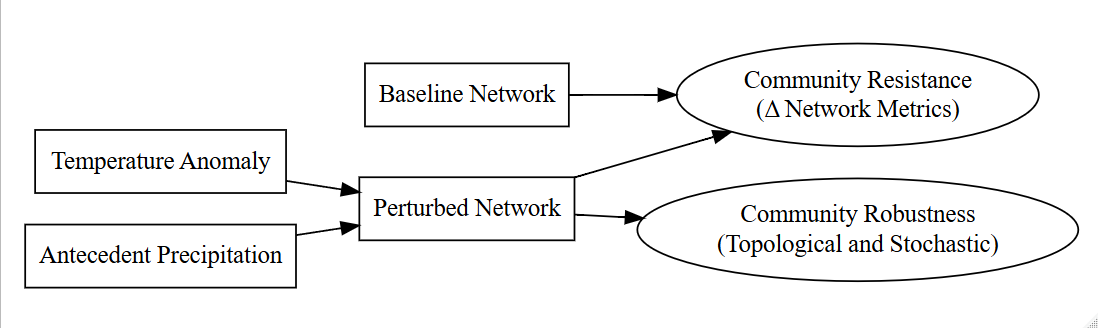
\includegraphics[width=0.9\textwidth]{SEM_diagram.png}
% % \end{figure}

% % \vspace{0.3cm}

% % \begin{itemize}
% %     \item Resistance shows weak and heterogeneous responses, suggesting partial decoupling from robustness.
% %     \item Climate variability (precipitation and temperature) alters interaction structure.
% %     \item \textbf{Moderate support:} precipitation contributes to increased robustness, but effects are context-dependent.
% %     \item Temperature effects are weak and primarily detected under stochastic dynamics (SCM).
% %     \item Results support a climate $\rightarrow$ stability pathway, but with strong mediation by network structure and extinction dynamics.
% % \end{itemize}

% % \end{frame}

% % % ------------------------------------------------
% % \begin{frame}{Main Questions Revisited}
% % \begin{itemize}
% %     \item \textbf{How does climate variability shape network structure?}
% %     \item Structural responses are evaluated indirectly using resistance, indicating climate effects on deviations from baseline network structure.
% %     \item \textbf{Do climate-driven structural changes alter stability?}
% %     \item Climate effects translate strongly into robustness, but only weakly into resistance.
% %     \item \textbf{Does extinction mechanism mediate climate effects?}
% %     \item Yes—extinction dynamics strongly condition climate sensitivity, with stronger effects when highly connected or dominant species are removed.
% % \end{itemize}
% % \end{frame}

% % % ------------------------------------------------
% % \begin{frame}{Mechanisms}
% % \begin{itemize}
% %     \item Water availability drives floral resources and interaction strength.
% %     \item Temperature anomalies may affect timing but not structure strongly.
% %     \item Extinction assumptions strongly influence robustness inference.
% % \end{itemize}
% % \end{frame}

% % % ------------------------------------------------
% % \begin{frame}{Broader Implications}
% % \begin{itemize}
% %     \item Stability depends on interaction structure, not just species richness.
% %     \item Robustness metrics are model-sensitive and should be compared carefully.
% %     \item Conservation should prioritize maintaining interaction networks.
% % \end{itemize}
% % \end{frame}

% % % ------------------------------------------------
% % \begin{frame}{Limitations}
% % \begin{itemize}
% %     \item Resistance depends on chosen network metrics.
% %     \item Robustness sensitive to extinction sequence assumptions.
% %     \item Climate variables may miss fine-scale microclimatic variation.
% % \end{itemize}
% % \end{frame}

% % % ------------------------------------------------
% % \begin{frame}{Take-Home Message}
% % \begin{itemize}
% %     \item Climate variability reshapes plant--pollinator stability primarily through precipitation-driven changes in interaction structure.
% %     \item Robustness is more sensitive than resistance and depends strongly on extinction dynamics.
% % \end{itemize}
% % \end{frame}


% \end{document}